\qrchapter{https://forgottenpillar.com/rsc/pl-fp-chapter21}{Pamiętając początek} \label{chap:remembering-the-beginning}

\egw{\textbf{Nie możemy ani na chwilę dopuścić do jakiegokolwiek \underline{błędnego przedstawienia} tych podniosłych i ważnych tematów prawdy, które stanowią wiarę naszego ludu od 1844 roku}}[Lt300-1903.9; 1903][https://egwwritings.org/read?panels=p7705.15]

Prawdziwe znaczenie \emcap{Fundamentalnych Zasad} to szersze spojrzenie na poselstwa trzech aniołów.

\egw{\textbf{Jesteśmy zachowującym przykazania ludem Bożym}. Przez ostatnie pięćdziesiąt lat była kierowana przeciwko nam każda forma herezji, aby \textbf{zaciemnić nasze umysły w odniesieniu do nauczania Słowa — \underline{szczególnie odnośnie do służby Chrystusa w niebiańskiej świątyni} i poselstwa niebios na te ostatnie dni, \underline{danego przez aniołów z czternastego rozdziału Księgi Objawienia}}. Poselstwa wszelkiego rodzaju i typu były narzucane Adwentystom Dnia Siódmego, aby \textbf{zastąpić prawdę, która punkt po punkcie} została odkryta przez pełne modlitwy studium i potwierdzona przez cudotwórczą moc Pana. \textbf{Lecz  drogowskazy, które uczyniły nas tym, czym jesteśmy, mają być zachowane i będą zachowane}, jak Bóg oznajmił przez swoje słowo i świadectwo swojego Ducha. \textbf{Wzywa nas, abyśmy trzymali się mocno, z uściskiem wiary, \underline{fundamentalnych zasad}, które są oparte na niepodważalnym autorytecie}}[SpTB02 59.1; 1904][https://egwwritings.org/read?panels=p417.299]

Tutaj widzimy, jak Ellen White opisała poselstwo \emcap{Fundamentalnych Zasad} jako poselstwa trzech aniołów z czternastego rozdziału Księgi Objawienia i jako poselstwo dotyczące służby Chrystusa w niebiańskiej świątyni. Pierwszy punkt \emcap{Fundamentalnych Zasad}, który jest tutaj szeroko omawiany, odpowiada na ważne pytanie zadane przez pierwszego anioła w czternastym rozdziale Księgi Objawienia: \textit{Kim jest Bóg, którego powinniśmy czcić}?

\bible{Bójcie się \textbf{Boga} i \textbf{oddajcie \underline{mu} chwałę}, gdyż \textbf{nadeszła godzina \underline{jego} sądu}. \textbf{Oddajcie cześć \underline{temu}}, który stworzył niebo i ziemię, morze i źródła wód}[Obj 14:7].

Kim jest Bóg, którego powinniśmy czcić, ogłoszony przez pierwszego anioła? Na przestrzeni czasu znajdujemy różne odpowiedzi na to pytanie. Dziś odpowiedzią jest Trójjedyny Bóg, czyli Trójca, jak przedstawiono w Fundamentalnych Wierzeniach Adwentystów Dnia Siódmego. Ale stawiamy pytanie: Kim był Bóg, którego czcili pionierzy adwentyzmu? Poselstwo pierwszego anioła jest związane z czasem proroczym, który wypełnił się za dni naszych pionierów. Całym celem ich pracy było głoszenie poselstw trzech aniołów. W 1844 roku nadeszła godzina Bożego sądu. Jeśli Bóg Trójca był Bogiem, którego godzina nadeszła, a nasi pionierzy nie czcili Trójcy, to czy nie minęli się z celem przy założeniu tego ruchu?

Zbadajmy historię naszego proroczego ruchu, mając na uwadze to pytanie: Czy nasi pionierzy czcili prawdziwego Boga, głosząc poselstwo pierwszego anioła? Czytamy wyjaśnienie wydarzeń przy upływie czasu w 1844 roku.

\egw{\textbf{Podobnie jak pierwsi uczniowie, William Miller i jego współpracownicy sami nie pojmowali w pełni znaczenia poselstwa, które głosili}. Błędy, które od dawna zakorzeniły się w Kościele, uniemożliwiały im dojście do poprawnej interpretacji ważnego punktu proroctwa. Dlatego chociaż głosili poselstwo, które Bóg im powierzył, aby przekazali je światu, to jednak z powodu błędnego zrozumienia jego znaczenia przeżyli rozczarowanie}[GC 351.2; 1888][https://egwwritings.org/read?panels=p132.1604]

\egwnogap{Wyjaśniając Księgę Daniela 8:14, «Aż do \textbf{dwóch tysięcy trzystu wieczorów i poranków. Wtedy \underline{świątynia zostanie oczyszczona}}», Miller, jak już wspomniano, przyjął powszechnie uznawany pogląd, że ziemia jest świątynią, i wierzył, że oczyszczenie świątyni oznacza oczyszczenie ziemi przez ogień przy przyjściu Pana. Gdy zatem odkrył, że koniec 2300 dni był wyraźnie przepowiedziany, doszedł do wniosku, że to ujawniało czas drugiego przyjścia. Jego błąd wynikał z przyjęcia powszechnego poglądu na temat tego, co stanowi świątynię}[GC 352.1; 1888][https://egwwritings.org/read?panels=p132.1607]

\egwnogap{W systemie typicznym, który był cieniem ofiary i \textbf{kapłaństwa Chrystusa}, \textbf{oczyszczenie świątyni było ostatnią służbą wykonywaną przez arcykapłana} w corocznym cyklu posługi. \textbf{Było to końcowe dzieło pojednania — usunięcie czy też oddalenie grzechu od Izraela}. \textbf{Zapowiadało to końcowe dzieło w posłudze naszego Arcykapłana w niebie, w usunięciu lub wymazaniu grzechów Jego ludu, które są zapisane w niebiańskich księgach}. \textbf{Ta służba obejmuje dzieło \underline{śledztwa, dzieło sądu}; i bezpośrednio poprzedza przyjście Chrystusa} w obłokach nieba z mocą i wielką chwałą; bo gdy On przyjdzie, każda sprawa będzie już rozstrzygnięta. Mówi Jezus: «Moja nagroda jest ze Mną, aby dać każdemu człowiekowi według jego uczynków». Obj 22:12. \textbf{To właśnie to dzieło sądu, bezpośrednio poprzedzające drugie przyjście, jest \underline{ogłoszone w poselstwie pierwszego anioła z Księgi Objawienia 14:7}: «Bójcie się \underline{Boga} i oddajcie Mu chwałę, \underline{gdyż nadeszła godzina Jego sądu}}»}[GC 352.2; 1888][https://egwwritings.org/read?panels=p132.1608]

\egwnogap{\textbf{Ci, którzy głosili to ostrzeżenie, przekazali właściwe poselstwo we właściwym czasie}. Lecz tak jak pierwsi uczniowie głosili: «Wypełnił się czas i przybliżyło się królestwo Boże», opierając się na proroctwie Księgi Daniela 9, podczas gdy nie dostrzegli, że śmierć Mesjasza była przepowiedziana w tym samym fragmencie Pisma, \textbf{tak Miller i jego współpracownicy głosili poselstwo oparte na \underline{Księdze Daniela 8:14 i Objawienia 14:7}, i nie dostrzegli, że były jeszcze inne poselstwa ukazane w Księdze Objawienia 14}, które również miały być głoszone przed przyjściem Pana. Tak jak uczniowie mylili się co do królestwa, które miało być ustanowione na końcu siedemdziesięciu tygodni, tak Adwentyści mylili się co do wydarzenia, które miało nastąpić po upływie 2300 dni. W obu przypadkach nastąpiło przyjęcie, a raczej przylgnięcie do popularnych błędów, które zaślepiły umysł przed prawdą. Obie grupy wypełniły wolę Bożą, przekazując poselstwo, które On pragnął, aby zostało przekazane, i obie, z powodu własnego niezrozumienia swojego poselstwa, przeżyły rozczarowanie}[GC 352.3; 1888][https://egwwritings.org/read?panels=p132.1609]

\begin{figure}[hp]
    \centering
    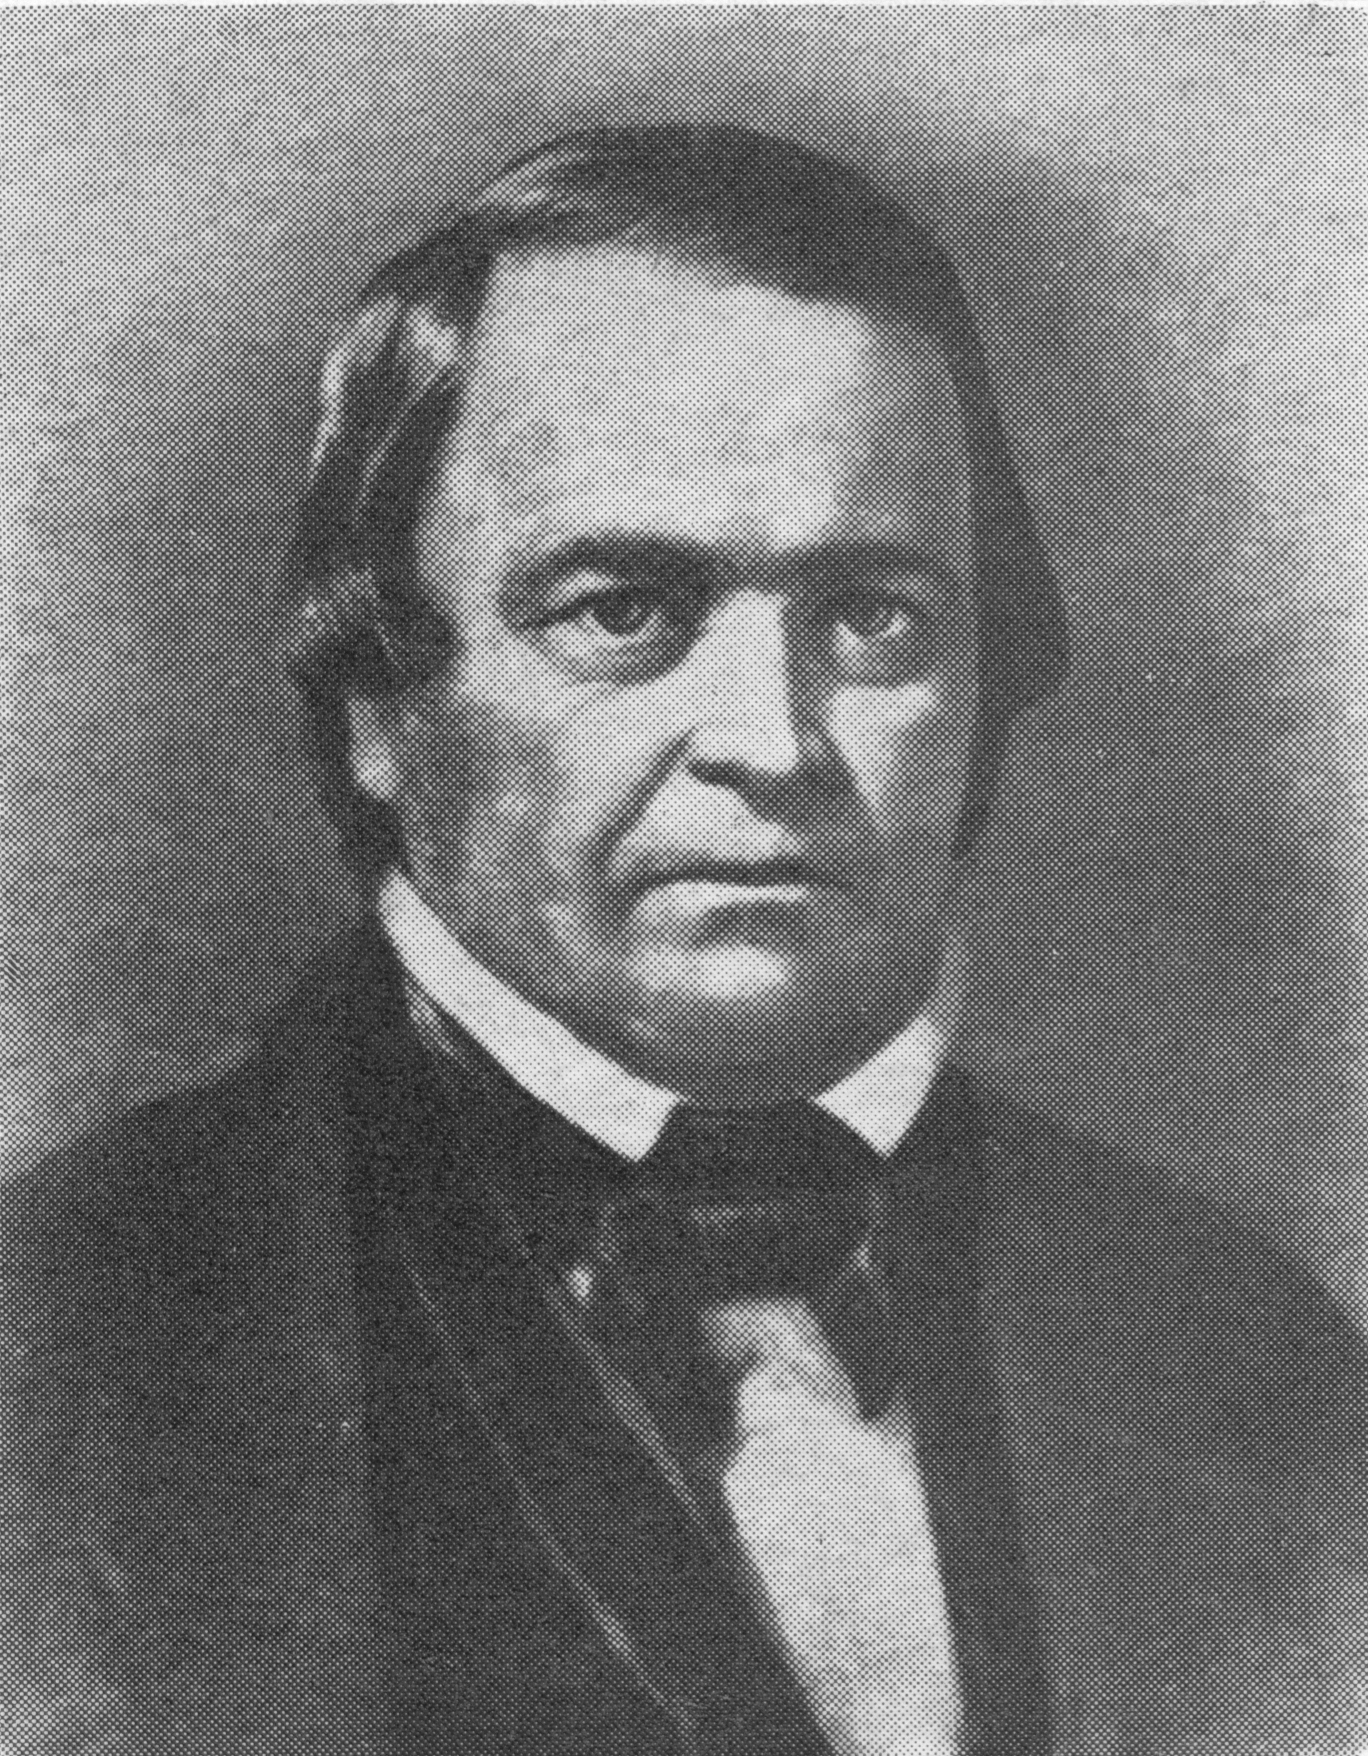
\includegraphics[width=1\linewidth]{images/william-miller.jpg}
    \caption*{William Miller (1782--1849)}
    \label{fig:w-miller}
\end{figure}

Czytając wyjaśnienie wielkiego rozczarowania, czy dostrzegłeś odpowiedź na pytanie: „\textit{Kim jest Bóg, którego sąd nadszedł}?” Pierwsze poselstwo anielskie z Obj 14:7 dokładnie pokrywa się z czasem proroczym ogłoszonym w Dn 8:14. Sąd, który nadszedł, był sądem śledczym, który rozpoczął się w 1844 roku. Biblia wyraźnie opisuje, czyja godzina sądu nadeszła w poselstwie pierwszego anioła. Przeczytajmy to w Biblii i zobaczmy komentarz Ellen White.

\egw{«Patrzyłem», mówi prorok Daniel, \textbf{«aż postawiono trony i \underline{zasiadł} \underline{Odwieczny}}: \textbf{Jego szata} była biała jak śnieg, a \textbf{włosy Jego głowy} jak czysta wełna; \textbf{Jego tron był ognistymi płomieniami}, a koła jego płonącym ogniem. Ognisty strumień wypływał i wychodził sprzed Niego: tysiąc tysięcy służyło Mu, a dziesięć tysięcy razy dziesięć tysięcy stało przed Nim: \textbf{\underline{sąd zasiadł i otwarto księgi}}». Dn 7:9--10, RV}[GC 479.1; 1888][https://egwwritings.org/read?panels=p132.2169]

\egwnogap{\textbf{Tak oto przedstawiono prorokowi w wizji wielki i uroczysty dzień, w którym charaktery i życie ludzi będą poddane przeglądowi przed Sędzią całej ziemi, a każdemu człowiekowi będzie oddane «według jego uczynków». \underline{Odwieczny to Bóg Ojciec}.} Mówi psalmista: «\textbf{Zanim} góry powstały, zanim ukształtowałeś ziemię i świat, \textbf{od wieków na wieki} \textbf{Ty jesteś Bogiem}». Ps 90:2. \textbf{\underline{To On, źródło wszelkiego bytu i źródło wszelkiego prawa, będzie przewodniczył w sądzie}}. A święci aniołowie jako słudzy i świadkowie, w liczbie «dziesięć tysięcy razy dziesięć tysięcy i tysiące tysięcy», uczestniczą w tym wielkim trybunale}[GC 479.2; 1888][https://egwwritings.org/read?panels=p132.2170]

\egwnogap{\textbf{«A oto ktoś podobny do \underline{Syna człowieczego} przybył z obłokami nieba, przyszedł do \underline{Odwiecznego}, i \underline{przyprowadzono Go przed Niego}}. I dano Mu panowanie, chwałę, i królestwo, aby wszystkie ludy, narody i języki Mu służyły: Jego panowanie jest wiecznym panowaniem, które nie przeminie». Dn 7:13--14. \textbf{Przyjście Chrystusa opisane tutaj nie jest Jego drugim przyjściem na ziemię}. \textbf{\underline{On przychodzi do Odwiecznego w niebie}, aby otrzymać panowanie, chwałę i królestwo}, \textbf{które zostaną Mu dane na zakończenie Jego dzieła jako pośrednika}. \textbf{\underline{To właśnie to przyjście, a nie Jego drugie przyjście na ziemię, było przepowiedziane w proroctwie, że nastąpi po zakończeniu 2300 dni w 1844 roku}}. \textbf{W towarzystwie niebiańskich aniołów nasz wielki Arcykapłan wchodzi do miejsca najświętszego i tam staje \underline{przed obliczem Boga}}, aby zaangażować się w ostatnie czynności swojej posługi na rzecz człowieka — \textbf{aby wykonać dzieło sądu śledczego} i \textbf{dokonać pojednania} za wszystkich, którzy okażą się uprawnieni do korzystania z jego dobrodziejstw}[GC 479.3; 1888][https://egwwritings.org/read?panels=p132.2171]

Odpowiedź jest prosta i bezpośrednia: Bogiem naszych pionierów był Przedwieczny. \egwinline{Odwieczny to Bóg Ojciec}. Jest On \textit{osobową}, \textit{duchową istotą}. Widzimy to w Jego opisie: \bible{którego szata była biała jak śnieg, a włosy jego głowy jak czysta wełna; jego tron był jak ognisty płomień, a jego koła jak płonący ogień}[Dn 7:9]. Przy zakończeniu proroctwa 2300 dni, w 1844 roku, \bible{nadeszła godzina Jego sądu}[Obj 14:7], \bible{zasiadł Odwieczny} i \bible{sąd zasiadł i otwarto księgi} [Dn 7:9--10]. Bóg z poselstwa pierwszego anioła jest Odwieczny. Nasi pionierzy nie byli ignorantami w kwestii prawdy o Bogu. Wierzyli, że \othersnodot{jest \textbf{jeden Bóg}, \textbf{\underline{osobowa, duchowa istota}}, \textbf{stwórca wszystkich rzeczy}, wszechmocny, wszechwiedzący i wieczny, nieskończony w mądrości, świętości, sprawiedliwości, dobroci, prawdzie i miłosierdziu; niezmienny i \textbf{\underline{wszędzie obecny przez swojego przedstawiciela, Ducha Świętego}}. Ps. 139:7}[Pierwszy punkt Fundamentalnych Zasad.]. Ten jeden Bóg to Ojciec, Odwieczny, \othersnodot{stwórca wszystkich rzeczy}, i mamy oddawać \bible{cześć Temu, który stworzył niebo i ziemię, morze i źródła wód}[Obj 14:7]. On \bible{stworzył wszystko przez Jezusa Chrystusa}[Ef 3:9].

Dziś poselstwo pierwszego anioła nie straciło nic na swoim znaczeniu. Poselstwo drugiego i trzeciego anioła zależą od pierwszego poselstwa i tylko pierwsze poselstwo wymaga działania z naszej strony. Mamy oddawać cześć Bogu. A dokładniej, mamy oddawać cześć właściwemu Bogu. W ostatnim i rozstrzygającym konflikcie będą dwa rodzaje czcicieli, jak poinformowano nas w Obj 13 i 14.

\bible{I wszyscy ci, którzy mieszkają na ziemi, będą \textbf{oddawać jej cześć} \normaltext{[bestii]}, \textbf{ci, których imiona nie są zapisane w księdze życia Baranka} zabitego od założenia świata}[Obj 13:8].

Grupa, która oddaje cześć bestii, otrzyma znamię bestii. Cały świat będzie zmuszony do oddawania czci bestii i jej obrazowi pod groźbą śmierci.

\bible{I miała \normaltext{[bestia]} moc, aby dać życie obrazowi bestii, tak żeby \textbf{obraz bestii} zarówno przemówił, jak i sprawił, aby \textbf{ci, którzy nie oddadzą czci obrazowi bestii, zostali zabici}}[Obj 13:15].

Nie powinniśmy uczestniczyć w tym kulcie. Uczmy się i miejmy wiarę jak trzej przyjaciele Daniela, którzy odmówili oddania pokłonu posągowi króla Nabuchodonozora. Bestia przedstawiona w Obj 13, która przymusza ludzkie sumienia pod groźbą śmierci, to papiestwo. Drogi przyjacielu, nie daj się zwieść. Papieski Bóg to Bóg Trójca. Nie przeocz tego.

Powinniśmy oddawać cześć Odwiecznemu, jak głosi poselstwo pierwszego anioła. To Bóg Stwórca, który stworzył wszystko przez swojego Syna, Jezusa Chrystusa. To Bóg z pierwszego punktu \emcap{Fundamentalnych Zasad}. Nasi pionierzy dobrze to rozumieli.

Prawdziwe zrozumienie misji i celu ruchu Adwentystów Dnia Siódmego powinno być przekonującym dowodem, że doktryna o Trójcy jest dla nas obcą doktryną. Znaleźliśmy się tam, gdzie jesteśmy dzisiaj, ponieważ zapomnieliśmy \egwinline{\textbf{drogę, którą Pan nas prowadził, oraz \underline{Jego nauki} w naszej dotychczasowej historii}}[LS 196.2; 1915][https://egwwritings.org/read?panels=p41.1083]. Bardzo smutno jest patrzeć, jak nasi adwentystyczni uczeni twierdzą, że nasi pionierzy nie rozumieli poprawnie doktryny o Bogu. Gdyby to była prawda, nasi pionierzy nie zdołaliby głosić poselstwa pierwszego anioła. Oni nie zawiedli. To my zawiedliśmy.

\othersnodot{\textbf{Większość założycieli adwentyzmu dnia siódmego nie mogłaby dziś przystąpić do Kościoła, gdyby musieli zaakceptować Fundamentalne Wierzenia denominacji. Dokładniej mówiąc, większość nie byłaby w stanie zgodzić się z wierzeniem numer 2, które dotyczy doktryny o Trójcy.} Dla Josepha Batesa doktryna o Trójcy była niebiblijną doktryną, dla Jamesa White'a była to «stara trynitarna niedorzeczność», a dla M. E. Cornella była owocem wielkiego odstępstwa, wraz z takimi fałszywymi doktrynami jak zachowywanie niedzieli i nieśmiertelność duszy}[G. R. Knight, \textit{Adventists and Change}, „Ministry Magazine”, październik 1993, s. 10.][https://www.ministrymagazine.org/archive/1993/10/adventists-and-change].

Doktryna o Trójcy jest doktryną, która podważa fundament naszej wiary, fundament, który został położony na początku naszego dzieła. Rozróżnienie między prawdą a błędem leży w hermeneutyce — metodzie interpretacji Biblii. Przeanalizujmy dokładnie tę kwestię.

\begin{titledpoem}

    \stanza{
        Gdy wiary światło zobaczyli, \\
        O Jego łaskę się modlili. \\
        Pionierzy wizje roztaczali, \\
        Boga już wtedy miłowali.
    }

    \stanza{
        Że sąd już nadszedł, wraz krzyczeli, \\
        Ogłosić bowiem światu mieli, \\
        Że to Odwieczny w nim zasiada, \\
        A nie pogańska bogów triada.
    }

    \stanza{
        Zaś Ellen White im opisała \\
        Widzenia nieba, które miała. \\
        Świątynia będzie oczyszczona, \\
        Miłość ma wielką Jezus do nas.
    }

    \stanza{
        Wraz z pierwszym aniołem wołali, \\
        Byśmy się Boga Stwórcy bali. \\
        „Którego Boga czcić to mamy?” — \\
        Nie trójcę, której nie poznamy.
    }

    \stanza{
        Pionierzy w Trójcę nie wierzyli, \\
        Bo w Słowo Boże się wpatrzyli. \\
        Odwieczny Ojciec, to wiedzieli, \\
        Innego Boga mieć nie chcieli.
    }

    \stanza{
        Dziś błędu szept się rozprzestrzenia, \\
        I z Trójcy trudno jest wyjść cienia. \\
        Jeśli ten bóg stoi zwycięsko, \\
        Stała się nasza misja klęską.
    }

    \stanza{
        Lecz to jest fałsz i rażący błąd, \\
        Którego trzeba się pozbyć stąd, \\
        By Bóg, co niegdyś był przez nich czczony \\
        Jako prawdziwy, był przywrócony.
    }

    \stanza{
        Wspólnie szukajmy oblicza Jego, \\
        By zyskać prawdę Boga naszego. \\
        W pionierskiej wizji musimy trwać, \\
        Na ich podstawach do końca stać.
    }

    \stanza{
        Czcijmy więc Boga, Sędziwego, \\
        I prawda niech na temat Jego \\
        Z trzecim aniołem w świat popłynie, \\
        I w mroku nocy nie zaginie.
    }

\end{titledpoem}

